\documentclass[12pt]{article}
\usepackage{times}
\usepackage[english]{babel}
\usepackage[utf8x]{inputenc}
\usepackage[colorinlistoftodos]{todonotes}
\usepackage[margin=1in]{geometry}
\usepackage{graphicx}
\usepackage{subcaption}
\usepackage{epstopdf}
\usepackage{cite}
\usepackage{listings}
\usepackage{dtklogos}
\usepackage{wrapfig}
\usepackage{amsmath}
\usepackage{amsthm}
\usepackage{amssymb}
\usepackage{amscd}
\usepackage{caption}
\usepackage{etoolbox}
\usepackage{fancyhdr}
\usepackage{stackengine}
\usepackage[export]{adjustbox}
\patchcmd{\thebibliography}{\section*{\refname}}{}{}{}
\usepackage[document]{ragged2e}    %This causes text to left align
\usepackage[colorlinks=true, linkcolor=black,citecolor=black,urlcolor=blue]{hyperref}
\bibliographystyle{IEEEtran}
\DeclareGraphicsRule{.tif}{png}{.png}{`convert #1 `dirname #1`/`basename #1 .tif`.png}

\title{MCHE 220: Report 2}

\begin{document}
\lefthyphenmin3
\righthyphenmin4
% \pretolerance=2000
% \tolerance=500 
% \emergencystretch=10pt
\raggedright     %Stops LaTeX from automatically hyphenating the right margin to fit better
%Combine this with \usepackage[document]{ragged2e} to get a text align left similar to natural MS Word
%-------------------------------------------------------------
%Header
%-------------------------------------------------------------
\fancyhf{}  
  \renewcommand{\headrulewidth}{0pt}
  \fancypagestyle{plain}{
    \fancyhead[R]{\thepage}} 
    \pagestyle{plain}
    
\captionsetup[table]{labelsep=space}

\begin{flushleft}
\hrulefill\\\hrule height 1pt
\vspace{5pt}
\textbf{TO: }William J. Emblom, Ph.D.  \hfill   \textbf{DATE: }\today                
\bigskip\\
\textbf{FROM: }Matthew J. Begneaud
\bigskip\\
\textbf{COPY: }N/A
\bigskip\\
\textbf{RE: }MCHE 220 Lab 2
\vspace{-10pt}
\end{flushleft}
\hrulefill \hrule height 1pt

%-------------------------------------------------------------
%Start of Paper
%-------------------------------------------------------------

\section*{\fontsize{12}{12}\selectfont INTRODUCTION}
This memorandum is being sent to Dr. Emblom to convey the analysis of a tensile test which took place on campus at University of Louisiana at Lafayette. The test was performed on two specimens, small metal rods, using a 60-ton Baldwin hydraulic machine press. The results of the test will be shown, as well as multiple plots of various data recorded and calculated from the experiment. These plots will be used to analyze the meaning of the data.
\bigskip


\section*{\fontsize{12}{12}\selectfont BACKGROUND}
The data collected from the test include forces recorded at various steps of the tensing, along with the corresponding length and diameter of the rods at that time. The original diameter and original length of the cylinder are also recorded. Using the given data, the engineering stress and engineering strain are both calculable. The engineering stress is defined as the force applied on an object divided by the original area of the face the force is applied normal to, as shown in (1). The engineering strain is defined as the change in length of an object per unit-length, as shown in (2).

\bigskip
\begin{equation}
\sigma = \frac{F}{A_{o}}
\end{equation}
\bigskip

\bigskip
\begin{equation}
\epsilon = \left | \frac{l_{o}-l}{l_{o}} \right |
\end{equation}
\bigskip

True stress is defined as the force applied on an object divided by the instantaneous area of the face that the force is applied normal to, and is calculable by (3). True strain is also calculable with the given data. According to [1], true strain is found by integrating the rate of the deformation tensor with respect to time, which results in (4).

\begin{equation}
\sigma_{T} = \frac {F}{A}
\end{equation}

\begin{equation}
\phi = \left | ln \frac{l}{l_{o}} \right |
\end{equation}
\bigskip


\bigskip


\section*{\fontsize{12}{12}\selectfont PROCEDURE}
The tensile test was conducted in the metal forming lab on UL Lafayette campus. The equipment used was a 60-ton Baldwin hydraulic press, two rods of unknown metal, a computer monitoring system to display the current force applied, and Vernier calipers to measure the length and diameter of each specimen as the test progressed. After creating two witness lines and recording the original length and diameter, a specimen was placed in the hydraulic machine press as shown in Figure 1. The increase in applied force was periodically stopped in order to record the current force, the distance between the two witness lines (change in length), and the diameter of the specimen. Both specimens were tensed until failure, upon which the specimens started necking and snapped as shown in Figure 2. After the data was collected, it was placed in an excel worksheet and converted to metric units. Calculations supplied additional information such as the original area, intermediate areas, engineering stress and strain, and true stress and strain.
\bigskip
\bigskip

% Figure 1
\begin{figure}[h!]  
  \centering
    \includegraphics[width=\linewidth]{specimen_in_machine.jpg}
    \caption{Specimen in Hydraulic Machine Press}
\end{figure}

\newpage

% Figure 2
\begin{figure}[h!]  
  \centering
    \includegraphics[width=3in, height=5in]{snapped_specimen2.jpg}
    \caption{Snapped Specimen After Failure}
\end{figure}


The force was plotted against the displacement (change in length) for each specimen and a trend-line was fitted to the plot for each specimen. The engineering stress was plotted against the engineering strain, as well as the true stress vs the true strain, for both specimens. The true stress was then plotted against the true strain again on a log-log graph and each specimen's curve was fitted with a power law trend-line.
\bigskip


\section*{\fontsize{12}{12}\selectfont RESLTS AND DISCUSSION}
The data recorded and calculated from the experiments is shown in Table 1 and Table 2. A plot shows how the force acting on each specimen correlated to the displacement in Figure 3. It is apparent for each specimen where failure started to occur by observing the sudden change in behavior of the material. For Specimen 1, the curve starts to flatten out towards the end, showing that the material started to elongate rapidly up until snapping. The same can be said for Specimen 2, where the slope of the curve starts to become negative at the end. This observation expresses that the material was stretching more easily, resulting in the tension in the rod to decrease. 

\newpage

% table1
\begin{center}
Table 1 
\\
\emph{Specimen 1 Data}
\\
\bigskip
\begin{tabular}{ c c c c c c c c }
\hline
Force & Length & Diameter & Area & Engr. Stress & Engr. Strain & True Stress & True Strain\\
(kN)    & (mm)   & (mm) &(mm$^2$)& (MPa)   & ---  & (MPa)   & ---    \\
\hline
0     & 25.00  & 7.99 & 50.265 & 0       & 0    & 0       & 0      \\
1.797   & 25.00  & 8.00 & 50.265 & 35.841  & 0    & 35.752  & 0      \\
4.274   & 25.00  & 8.00 & 50.265 & 94.217  & 0    & 93.981  & 0      \\
6.500   & 25.25  & 7.99 & 50.140 & 129.614 & 0.01 & 129.614 & 0.0099 \\
8.514   & 20.25  & 7.98 & 50.014 & 169.803 & 0.01 & 170.229 & 0.0099 \\
9.020   & 25.50  & 7.96 & 49.764 & 179.916 & 0.02 & 181.275 & 0.0198 \\
14.577  & 25.50  & 7.90 & 49.017 & 290.723 & 0.02 & 297.385 & 0.0198 \\
20.297  & 26.00  & 7.90 & 49.017 & 404.812 & 0.04 & 414.088 & 0.0392 \\
23.020  & 27.00  & 7.73 & 46.930 & 459.106 & 0.08 & 490.510 & 0.0770 \\
24.136  & 29.00  & 7.54 & 44.651 & 481.374 & 0.16 & 540.547 & 0.1484 \\
24.639  & 31.00  & 6.94 & 37.828 & 491.399 & 0.24 & 651.342 & 0.2151 \\
\hline
\end{tabular}
\end{center}

\bigskip
\bigskip
\bigskip

% table2
\begin{center}
Table 2 
\\
\emph{Specimen 2 Data}
\\
\bigskip
\begin{tabular}{ c c c c c c c c }
\hline
Force & Length &  Diameter & Area & Engr. Stress & Engr. Strain & True Stress & True Strain\\
(kN)   & (mm) & (mm) &(mm$^2$)& (MPa)  & ---  & (MPa)   & ---    \\
\hline
0     & 50.00 & 7.85 & 48.460 & 0      & 0    & 0       & 0      \\
0.524 & 50.00 & 7.90 & 49.017 & 10.831 & 0    & 10.708  & 0      \\
0.676 & 50.00 & 7.88 & 48.769 & 13.952 & 0    & 13.864  & 0      \\
1.049 & 50.00 & 7.84 & 48.275 & 21.663 & 0    & 21.746  & 0      \\
1.992 & 50.00 & 7.84 & 48.275 & 41.123 & 0    & 41.280  & 0      \\
2.931 & 50.50 & 7.83 & 48.152 & 60.491 & 0.01 & 60.878  & 0.0099 \\
3.558 & 51.00 & 7.73 & 46.930 & 73.433 & 0.02 & 75.828  & 0.0198 \\
4.038 & 52.50 & 7.65 & 45.963 & 83.347 & 0.05 & 87.874  & 0.0488 \\
4.288 & 54.50 & 7.52 & 44.415 & 88.487 & 0.09 & 96.547  & 0.0862 \\
4.452 & 56.75 & 7.39 & 42.892 & 91.884 & 0.14 & 103.811 & 0.1266 \\
4.501 & 59.00 & 7.27 & 41.511 & 92.893 & 0.18 & 108.445 & 0.1655 \\ 
4.541 & 61.00 & 7.14 & 40.039 & 93.719 & 0.22 & 113.429 & 0.1988 \\
4.314 & 63.00 & 6.03 & 28.558 & 89.038 & 0.26 & 151.089 & 0.2311 \\
3.193 & 65.00 & 4.30 & 14.522 & 65.906 & 0.30 & 219.930 & 0.2623 \\
1.734 & 67.50 & 3.04 & 7.258  & 35.799 & 0.35 & 239.009 & 0.3001 \\
\hline
\end{tabular}
\end{center}

\newpage

% Figure 3
\begin{figure}[h!]  
  \centering
    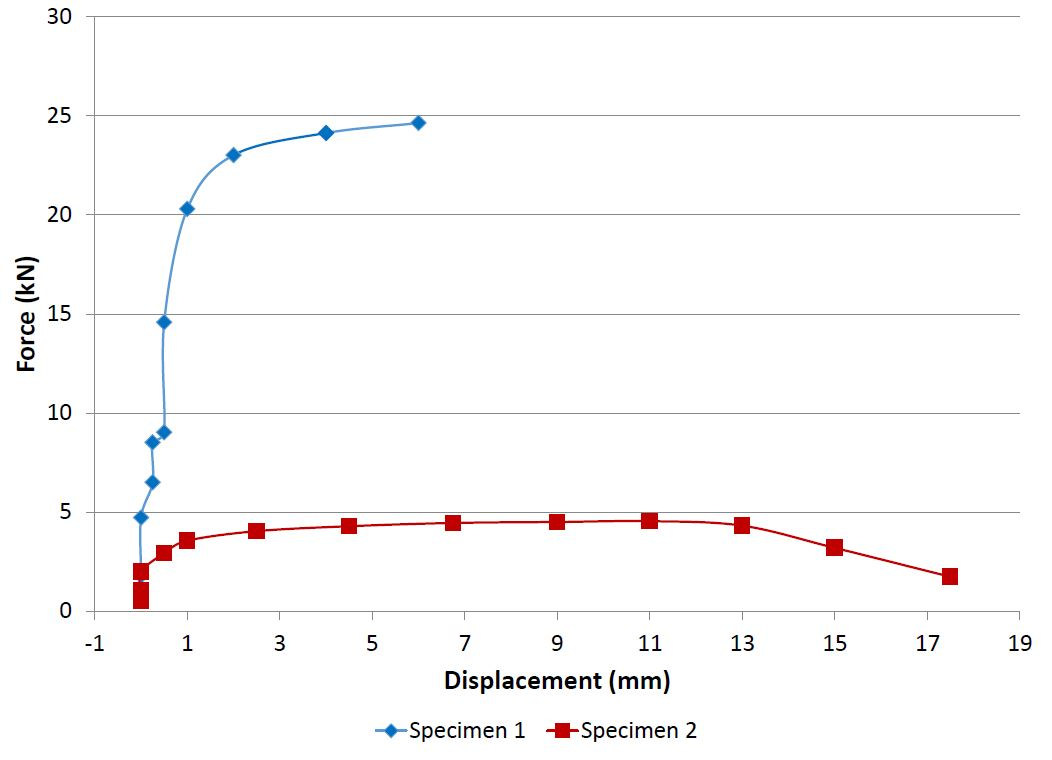
\includegraphics[width=\linewidth,height=4.2in]{force_vs_displacement.JPG}
    \caption{Force vs Displacement}
\end{figure}

The engineering stress and strain are plotted in Figure 4 for both specimens. The true stress and strain are plotted for each specimen in Figure 5. Specimen 1's engineering ultimate stress occurs around (0.26, 500MPa), while its true ultimate stress occurs around (0.1, 500MPA). Specimen 2's engineering ultimate stress occurs around (0.2, 95 MPa), while its true ultimate stress occurs around (0.18, 110 MPa). Comparing the plots from Figure 4 and Figure 5, it is seen that the ends of the data curves tend to have a sudden rise in the true stress and strain plot, whereas the engineering stress and strain do not show this behavior. This is because a true stress-strain diagram shows that a material really experiences an increasing stress as it is tensed, because the area of necking rapidly decreases in size, causing the stress to be higher [2]. Engineering stress-strain diagrams, however, tend to show a drop in stress near failure, because in reference to the original area, the stress would be decreasing when the material begins to yield.
\bigskip

Engineering stress does not account for the change in area of the cylinder as it stretches. Since only the original area is considered in the engineering stress, the result is a lower-than-realistic stress calculation for tension, because in reality the area decreases as the specimen stretches. For a material under compression, the stress would be overestimated rather than underestimated since the area would be increasing in reality. True stress considers the change in area as the cylinder compresses [3], which provides more accurate results. It should be noted that because of this difference, engineering stress and strain should only be used for analysis in cases where the deformation of the object in question is negligible. This entails any case where the forces on a member are not enough to bring the material to its yield point. Otherwise, True stress and strain should be used for analysis.

\newpage

% Figure 4
\begin{figure}[h!]  
  \centering
    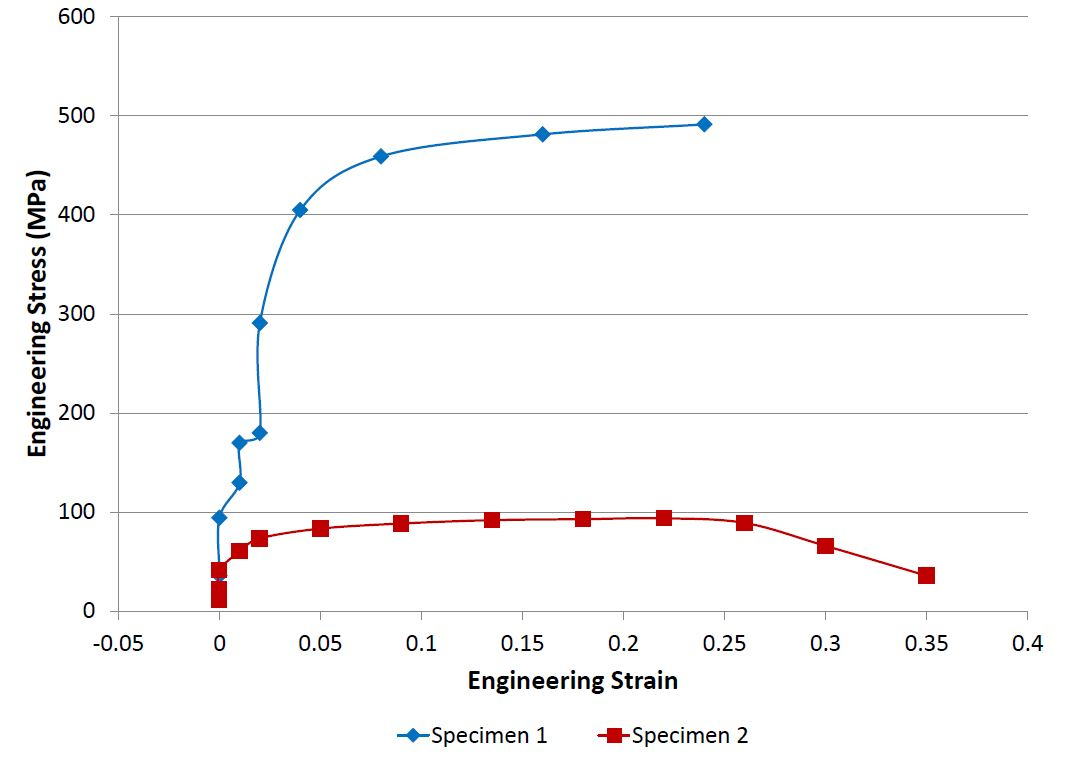
\includegraphics[width=5.5in,height=3.8in]{engr_stress_vs_engr_strain.JPG}
    \caption{Engineering Stress vs Engineering Strain}
\end{figure}

% Figure 5
\begin{figure}[h!]  
  \centering
    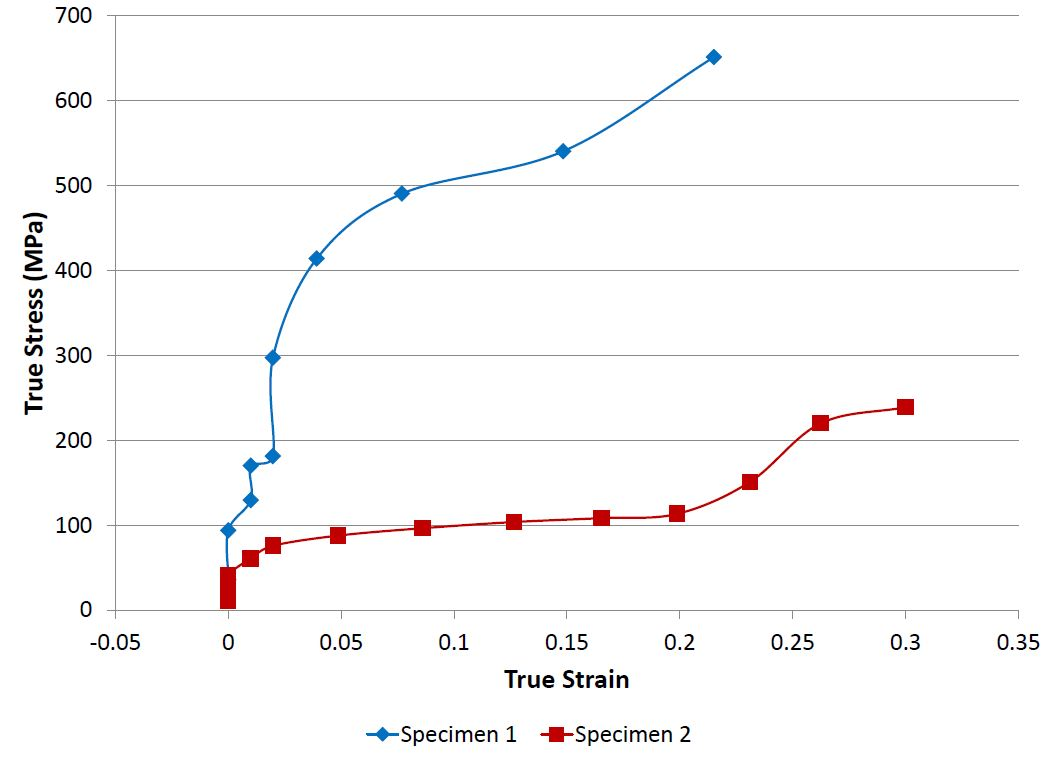
\includegraphics[width=5.5in,height=3.8in]{true_stress_vs_true_strain.JPG}
    \caption{True Stress vs True Strain}
\end{figure}

\newpage

The true stress and strain are also plotted on a log-log scale and fitted with trend lines, shown in Figure 6. The data points near failure are excluded in order to show the more predictable range of tension before the material hits its yield point. At the yield point, the material starts to stretch and elongate more easily, requiring significantly less force to increase the strain [4]. Also, the plot does not show the behavior of the material near a stress or strain value of zero since zero has no logarithm (i.e. zero does not exist in the logarithmic scale). 
\bigskip

The trend-line used to fit each specimen is a power law curve. Notice that the power law trend-lines look linear in a log-log scale. This is because the slope for the power law curve is expressed as an equation consisting solely of logarithmic functions, as seen in (5). Since the slope is logarithmic in nature, it appears linear on a log-log scale. 
\bigskip

\begin{equation}
B = \frac{ln\sigma_{1}-ln\sigma_{2}}{ln\phi_{1}-ln\phi_{2}}
\end{equation}

\bigskip
\bigskip
\bigskip

% Figure 6
\begin{figure}[h!]  
  \centering
    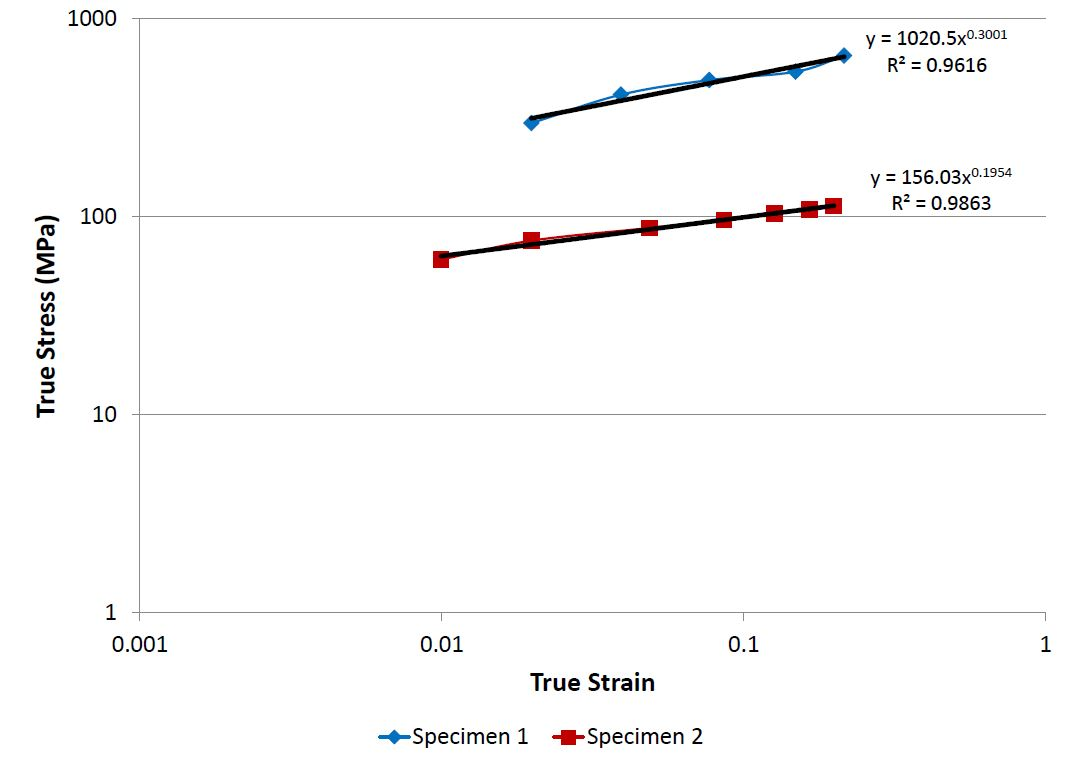
\includegraphics[width=\linewidth]{true_stress_vs_true_strain_log.JPG}
    \caption{True Stress vs True Strain (Log-Scale)}
\end{figure}

\newpage

A more extensive and accurate tensile test performed on a sample of A6111-T4 aluminum can be seen in Figure 7 and Figure 8. The engineering stress-strain diagram is shown in Figure 7, while the true stress-strain diagram is shown in Figure 8. The curves are smoother and more accurate due to collecting an extensive amount of data points. Both diagrams have points labeled, which include the proportional limit, yield stress, and ultimate stress. These diagrams are a much better representation of material behavior thanks to the extensive measures taken during the tensile test.

\bigskip

% Figure 7
\begin{figure}[h!]  
  \centering
      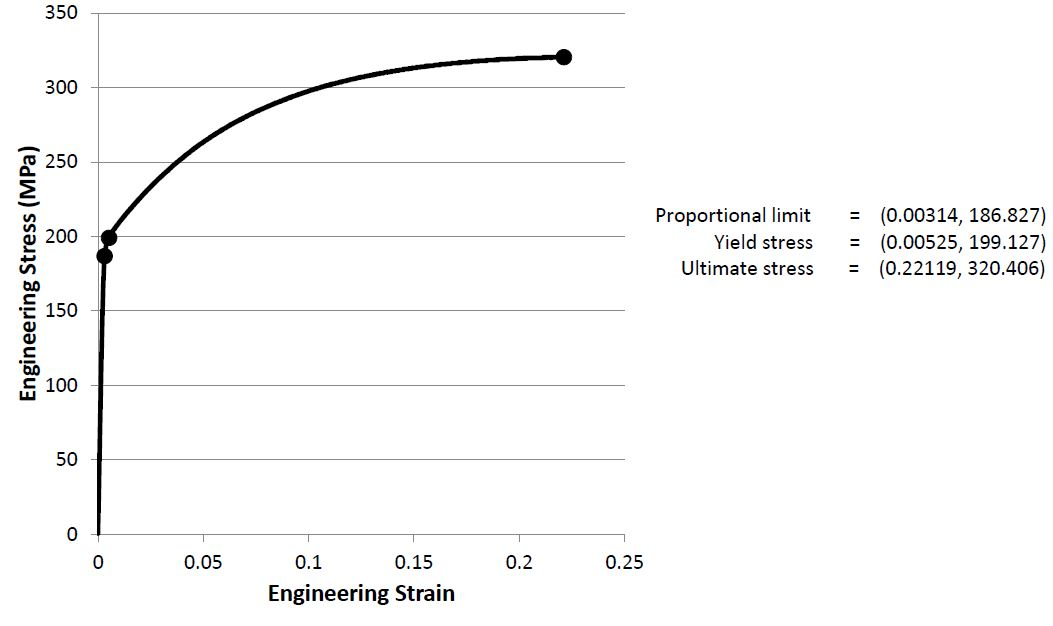
\includegraphics[width=5in,height=3in]{emblom_engr.JPG}
      \caption{Engineering Stress vs Engineering Strain (A6111-T4 aluminum)}
\end{figure}

\bigskip
\bigskip

% Figure 8
 \begin{figure}[h!]
   \centering
       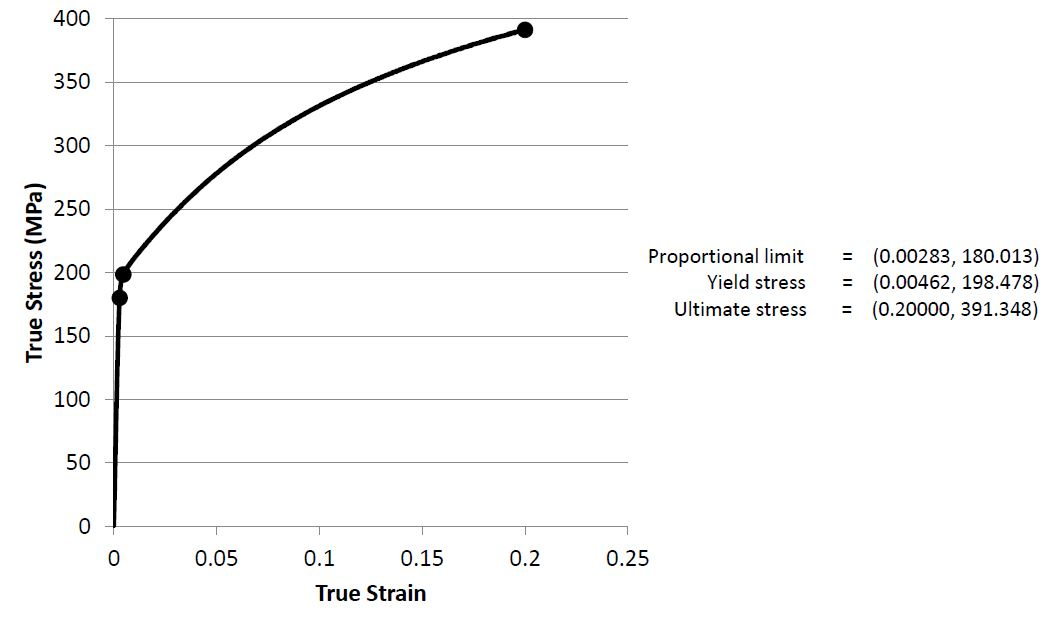
\includegraphics[width=5in,height=3in]{emblom_true.JPG}
         \caption{True Stress vs True Strain (A6111-T4 aluminum)}
\end{figure}


\newpage

The true stress and strain analysis give more accurate values than the engineering stress and strain. This is because the instantaneous dimensions are considered in true stress and strain calculations, rather than just the original dimensions as in engineering stress calculations. Since the two types of stress and strain behave similarly up to the yield point where deformation begins to occur, it is recommended that engineering stress and strain only be used for analysis regarding members that are not loaded enough to cause any deformation. If deformation is to occur in the range of loading considered for a member, true stress and strain should be used. 
\bigskip

\section*{\fontsize{12}{12}\selectfont CONCLUSION}
The data from this tensile test, performed on UL campus, has been analyzed and plotted. The originally recorded data was also used to calculate the engineering stress and strain, as well as the true stress and strain. The results showed that true stress and strain tend to follow a power law trend when plotted against each other on a log-log scale, which was shown in Figure 8. A more extensive test was also performed on A6111-T4 aluminum which resulted in very accurate engineering and true stress-strain diagrams. These diagrams further demonstrate the relation between stress and strain, as well as the difference between engineering stress and strain, and true stress and strain.
\bigskip

The data also shows that the true stress was higher than the engineering stress, which is due to the fact that true stress involves the instantaneous area of a material during loading, while engineering stress only uses the original area. This difference also results in the true strain being lower than the engineering strain. Thus, it has been concluded that engineering stress and strain should only be used for analysis when the forces present on an object do not bring the material past its yield point where deformation begins to occur. If the forces on the object cross into the range where deformation occurs, true stress and strain should be used for analysis to achieve higher accuracy.
\bigskip


\section*{\fontsize{12}{12}\selectfont REFERENCES}

\begin{thebibliography}{2}

\bibitem{McGinty}
Mcginty, B., n.d.,
"True Strain," \emph{Continuum Mechanics}, from
http://www.continuummechanics.org/

\bibitem{}
Hibbeler, R.C., 2014, \emph{Mechanics of Materials}, Prentice Hall, Upper Saddle River, NJ, Chap. 3.

\bibitem{}
“True Stress versus Engineering Stress,” \emph{Engineering Quality Solutions}, n.d., from
http://www.eqsgroup.com/all-about-steel/difference-between-true-stress-and-engineering-stress.asp

\bibitem{}
"Tensile Properties," \emph{NDT Resource Center}, n.d., from
\\https://www.nde$-$ed.org/EducationResources/CommunityCollege/Materials/Mechanical/Tensile.htm

\end{thebibliography}

%\section*{\fontsize{12}{12}\selectfont APPENDIX}

%\begin{table}[h!]
%  \caption{}
%  \includegraphics[width=\linewidth]{table1.png}
%\end{table}

\end{document}
----------------------------%TEmplates-------------------------------

-------------------------Figure-----------------------

\begin{figure}[h!]  
  \centering
    \includegraphics[width=\linewidth]{**file**}
    \caption{Docking Station}
\end{figure}

---------------------------Table-----------------------
\begin{table}[ht]
\caption{Nonlinear Model Results} % title of Table
\centering % used for centering table
\begin{tabular}{c c c c} % centered columns (4 columns)
\hline\hline %inserts double horizontal lines
Case & Method\#1 & Method\#2 & Method\#3 \\ [0.5ex] % inserts table
%heading
\hline % inserts single horizontal line
1 & 50 & 837 & 970 \\ % inserting body of the table
2 & 47 & 877 & 230 \\
3 & 31 & 25 & 415 \\
4 & 35 & 144 & 2356 \\
5 & 45 & 300 & 556 \\ [1ex] % [1ex] adds vertical space
\hline %inserts single line
\end{tabular}
\label{table:nonlin} % is used to refer this table in the text
\end{table}



probably best to insert as an image from excel

\bigskip\\
\begin{table}[h!]
  \caption{}
  \includegraphics[width=\linewidth]{**file**}
\end{table}
\bigskip\\





-----------------------------Equations------------------------
-----------------------------Regular
\begin{equation}
a = b + c
\end{equation}

--------------------------------- Multiline
\begin{multline}
a = b + c + d + e + f
+ g + h + i + j \\
+ k + l + m + n + o
\end{multline}

-------------------------------Citations-------------------------
\bibitem{Author last name}
  Last, First., year of publication,
  article name, book(etc) name, from \\
  link goes here

----------------------------------other-----------------------------

equations:
http://moser-isi.ethz.ch/docs/typeset_equations.pdf

citations:
http://library.missouri.edu/engineering/about/guides/asme
https://www.asme.org/shop/proceedings/conference-publications/references